
\section{Primeira Questão (6 pts)}

\subsection{Análise Analítica}

\numberwithin{equation}{section}
\numberwithin{figure}{section}

Um fluido de viscosidade $\mu$ e massa específica $\rho$ está em repouso
sobre uma placa horizontal quando ela começa a se mover com velocidade constante
$U_0$. A Figura \ref*{fig:geometriaQ1} exibe a geometria do problema.


\begin{figure}[h!]
    \caption{Geometria da questão 1.}
    \label{fig:geometriaQ1}
    \centering
    \centerline{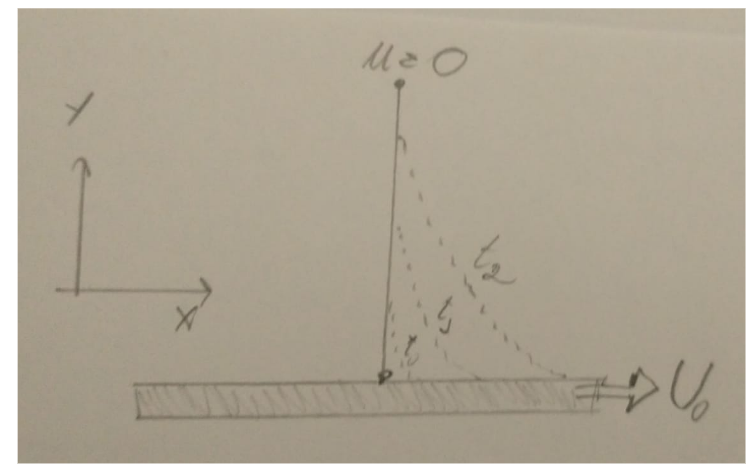
\includegraphics[scale=0.35]{geometriaQ1.png}}
    \par{Fonte: elaboração própria.}
\end{figure}

Como mostra a Figura \ref*{fig:geometriaQ1}, a linha média do fluido começa
a ser arrastada pelo movimento da placa, e a cada instante de tempo $t_0$,
$t_1$ e $t_2$ o movimento da placa atinge pontos cada vez mais altos
da linha média do fluido. Nesse cenário, a velocidade horizontal $u$ do
fluido é uma função de duas variáveis: posição vertical $y$ e tempo $t$.

A equação diferencial que modela o problema é

\begin{equation}\label{eq:modeloQ1}
    \diffp{u}{t} = \frac{\mu}{\rho} \diffp[2]{u}{y}
\end{equation}

\noindent com as seguintes condições de contorno:

\begin{equation}\label{eq:modeloQ1Contorno}
    \begin{cases}
        u(0, t) = U_0, & 0 \leq t \leq T \quad \textrm{Cond. contorno 1}\\
        u(H, t) = 0,   & 0 \leq t \leq T \quad \textrm{Cond. contorno 2}\\
        u(y, 0) =  0,  & 0 < y \leq H \quad \textrm{Cond. inicial}     \\
    \end{cases}
\end{equation}

Veja que o problema é modelado por uma equação diferencial de segunda ordem
em regime transiente, logo precisamos de duas condições de contorno e uma condição
inicial. Estamos analisando apenas o que acontence com a linha média, logo temos 
apenas uma dimensão de análise $y$.

No nosso sistema de coordenadas, $y = 0$ corresponde ao ponto do fluido
em contato com a placa, e $y = H$ é a altura máxima que iremos considerar na análise.
Note que, para $H$ suficientemente grande, faz sentido assumir que o movimento da placa
não atinge esses pontos do fluido a uma grande distância da placa, de modo que
$u(H, t) = 0$. O tempo total de análise é dado por $T$.

O problema modelado por \eqref{eq:modeloQ1} e \eqref{eq:modeloQ1Contorno} possui solução analítica dada por

\begin{equation}\label{eq:solAnaliticaQ1}
    u(y,t) = U_0 \left[1 - erf\left(\frac{y}{2\sqrt{\frac{\mu}{\rho}t}}\right)\right]
\end{equation}

\noindent em que $erf$ é a função erro definida como

\begin{equation}\label{eq:erf}
    erf(\beta) = \frac{2}{\sqrt{\pi}} \int_0^\beta e^{-x^2} \, dx
\end{equation}

Usando linguagem R e a IDE RStudio,
é possível obter a distribuição de velocidades do fluido
a partir da equação \eqref{eq:solAnaliticaQ1}, uma vez que a função erro $erf$
já está implementada em pacotes da linguagem. Usamos os seguintes parâmetros:

\begin{itemize}
    \item Domínio de análise vertical: $H=10 \un{cm}$
    \item Domínio de análise no tempo: $T=1 \un{s}$
    \item Viscosidade: $\mu=0.29 \un{ kg m$^{-1}$ s$^{-1}$}$
    \item Massa específica: $\rho=891 \un{kg m$^{-3}$}$
    \item Velocidade da placa: $U_0 = 1 \un{m/s}$
\end{itemize}

A Figura \ref*{fig:velocidadesAnaliticaQ1}
exibe os valores de $u(y,t)$ em função do tempo e posição vertical obtidos através da equação
\eqref{eq:solAnaliticaQ1} com os parâmetros acima.

\begin{figure}[h!]
    \caption{Velocidade $u$ do fluido em função da posição e tempo.}
    \label{fig:velocidadesAnaliticaQ1}
    \centering
    \centerline{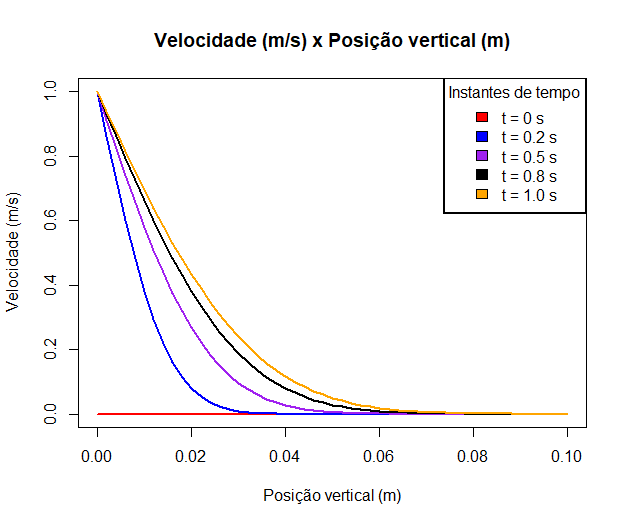
\includegraphics[scale=0.5]{velocidadesAnaltico.png}}
    \par{Fonte: elaboração própria.}
\end{figure}

As velocidades obtidas analiticamente na Figura \ref*{fig:velocidadesAnaliticaQ1} são condizentes
com o analisado da geometria na Figura \ref*{fig:geometriaQ1}. Conforme o tempo passa,
os pontos do fluido apresentam velocidade $u$ cada vez maior, uma vez que são arrastados
pelo movimento da placa. Os pontos em $y > 7 \un{cm}$ já não sofrem nenhum efeito
do movimento da placa até $t = 1 \un{s}$.

Analisando os pontos específicos pedidos no exercício, temos

\[ u(3 \un{cm}, 0.5 \un{s}) = 0.0963 \un{m/s} \]
\[ u(3 \un{cm}, 1 \un{s}) = 0.2396 \un{m/s} \]

\subsection{Análise Numérica}

Uma vez entendido o que está acontecendo analiticamente, podemos fazer uma análise
numérica do problema usando o método de diferenças finitas. O primeiro passo
é discretizar a equação diferencial \eqref{eq:modeloQ1}, trocando os diferenciais
por diferenças.

\begin{equation}\label{eq:modeloQ1Discretizado}
    \frac{u^{p+1} - u^p}{\Delta t} = \frac{\mu}{\rho} \frac{u_{i+1} - 2u_i + u_{i-1}}{\left(\Delta y\right)^2}
\end{equation}

Em \eqref{eq:modeloQ1Discretizado} adotamos a seguinte simbologia:

\begin{itemize}
    \item Sobrescrito $p$: indica o tempo da velocidade $u$. $p$ indica o tempo atual, $p + 1$ o próximo tempo
    \item Subscrito $i$: indica a posição vertical da velocidade $u$. $i$ indica a posição atual, $i + 1$ a próxima posição
    \item $\Delta t$: intervalo de discretização no tempo
    \item $\Delta y$: intervalo de discretização no espaço (vertical)
\end{itemize}

Assim, a linha média da Figura \ref*{fig:geometriaQ1} é discretizada em $H / \Delta y$ elementos de
comprimento $ \Delta y$, e o tempo é transcorrido a partir de $t = 0$ até $t = T$ em intervalos de
$ \Delta t$. Vamos reescrever \eqref{eq:modeloQ1Discretizado} de modo a expressar a
velocidade futura em função da velocidade antiga.

\begin{equation}\label{eq:Q1explicito}
    u^{p+1} = u^p + \frac{\mu}{\rho} \frac{\Delta t}{\left(\Delta y\right)^2} \left(u_{i+1}^p - 2u_i^p + u_{i-1}^p\right)
\end{equation}

Em \eqref{eq:Q1explicito}, usamos o método explícito ao aplicar as difenças finitas. Portanto,
é fundamental analisar os critérios de estabilidade para que a solução converja. Em transferência
de calor, vimos que a equação diferencial de condução unidimensional em regime transiente é

\begin{equation}\label{eq:transCalTransiente}
    \frac{1}{\alpha} \diffp{T}{t} = \diffp[2]{T}{y} \logo \diffp{T}{t} = \alpha \diffp[2]{T}{y}
\end{equation}

\noindent onde $\alpha$ é a difusividade térmica do material. Nesse modelo, o critério de estabilidade
é, segundo Incropera (2007),

\begin{equation}\label{eq:transCalestabilidade}
    \frac{\alpha \Delta t}{\left(\Delta y\right)^2} \leq \frac{1}{2}
\end{equation}

Comparando as equações diferenciais \eqref{eq:modeloQ1} e \eqref{eq:transCalTransiente},
podemos ver que as constantes $\alpha$ e $\mu / \rho$ possuem o mesmo papel, apesar de uma
ter um significado físico de transferência de calor e outra um significado de mecânica dos fluidos.
Nesse sentido, podemos inferir que o critério de estabilidade de \eqref{eq:Q1explicito} é

\begin{equation}\label{eq:Q1estabilidade}
    \frac{\mu}{\rho} \frac{\Delta t}{\left(\Delta y\right)^2} \leq \frac{1}{2}
\end{equation}

Concluída essa análise, podemos jogar \eqref{eq:Q1explicito} no computador para obter a solução
numérica do problema. Novamente usando R e a IDE RStudio, o pseudocódigo abaixo mostra
o procedimento para resolver o problema numericamente.

\begin{algorithmic}
    \State listaSoluções $\gets$ Lista()
    \State $i \gets 0$
    \For{\texttt{$\Delta t$ em $T$}}
        \State soluçãoAntiga $\gets$ listaSoluções[$i$]

        \For{\texttt{$\Delta y$ em $H$}}
            \State calcule novasVelocidades
        \EndFor

        \State $i \gets i + 1$
        \State listaSoluções[$i$] $\gets$ novasVelocidades
    \EndFor

    \Return listaSoluções
\end{algorithmic}

O pseudocódigo acima está bastante simplificado, mas ele mostra a ideia principal: percorremos 
dois loops, um para o tempo e um para a posição vertical. Percorremos todos os intervalos verticais,
calculando a velocidade em cada nó, para cada intervalo de tempo. Ao final de cada loop do tempo, salva o novo
vetor de velocidades calculado na lista de soluções. No final da execução, a lista de soluções 
tem $T / \Delta t$ elementos, e cada elemento é um vetor de tamanho $H / \Delta y$.

O código completo desenvolvido em R, que implementa o pseudocódigo acima,
pode ser visto no ANEXO A. A Figura \ref*{fig:tabelaNumericaQ1} mostra a distribuição de 
velocidades obtida com o código do ANEXO A para $\Delta t = 0.05 \un{s}$ e $\Delta y = 1 \un{cm}$.

\begin{figure}[h!]
    \caption{Distribuição de velocidades obtida com a solução numérica.}
    \label{fig:tabelaNumericaQ1}
    \centering
    \centerline{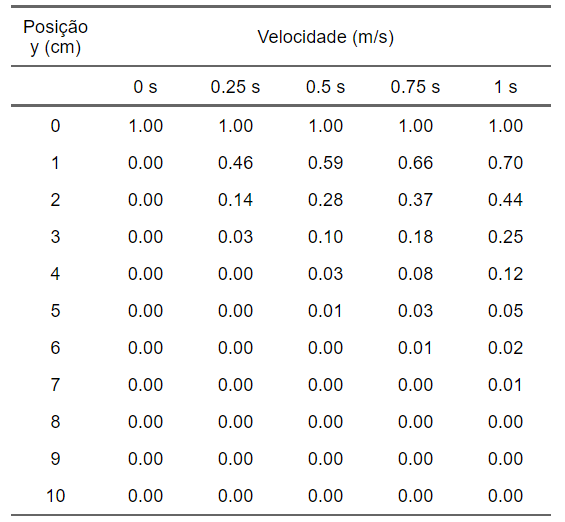
\includegraphics[scale=0.75]{tabelaNumericaQ1.png}}
    \par{Fonte: elaboração própria.}
\end{figure}

Note que os valores escolhidos de $\Delta t$ e $\Delta y$ atendem ao critério de estabilidade:

\[ \frac{\mu}{\rho} \frac{\Delta t}{\left(\Delta y\right)^2} = 0.1627 \leq 0.5 \]

A tabela da Figura \ref*{fig:tabelaNumericaQ1} foi construída com o pacote  \verb|flextable| da linguagem,
que formata a lista de soluções na forma de uma tabela.  

Os dados obtidos na Figura \ref*{fig:tabelaNumericaQ1} são condizentes tanto com o esperado da geometria
quanto com o resultado analítico da Figura \eqref{fig:velocidadesAnaliticaQ1}. Com o passar no tempo,
as velocidades mais distantes da placa aumentam, e pontos muito distantes não sofrem efeito 
algum.

Em particular, na Figura \ref*{fig:tabelaNumericaQ1}, obtemos 

\[ u(3 \un{cm}, 0.5 \un{s}) = 0.1049 \un{m/s} \]
\[ u(3 \un{cm}, 1 \un{s}) = 0.2455 \un{m/s} \]

\noindent através da solução numérica. É importante destacar que na Figura \ref*{fig:tabelaNumericaQ1}
os valores foram arrendondados para a segunda casa decimal para facilitar a leitura.
O erro percentual com a solução analítica é dado por 

\begin{equation}\label{eq:erroPercentual}
    E_{\%} = \frac{V_{\un{numerico}} - V_{\un{analitico}}}{V_{\un{analitico}}} 100\%
\end{equation}

Assim, para $y = 3 \un{cm}$ em $t = 0.5 \un{s}$ temos erro  

\[ E_{\%} = \frac{0.1049 - 0.0963}{0.0963} 100\% = 8.9\% \]

\noindent e para $y = 3 \un{cm}$ em $t = 1 \un{s}$,

\[ E_{\%} = \frac{0.2455 - 0.2396}{0.2396} 100\% = 2.5\% \]

\noindent com ambos erros inferiores a $10\%$ em relação ao resultado analítico. Podemos recalcular
esses valores para diferentes malhas, isto é, para diferentes valores de $\Delta t$ e
$\Delta y$. No software, basta alterar as variáveis no início do código e refazer
a simulação. A Figura \ref*{fig:testeDeMalhas} mostra o resultado desse teste de malhas.

\begin{figure}[h!]
    \caption{Erros percentuais com a solução analítica para diferentes malhas.}
    \label{fig:testeDeMalhas}
    \centering
    \centerline{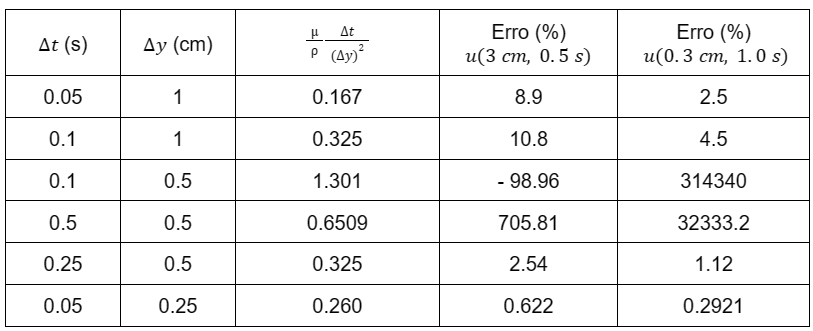
\includegraphics[scale=0.50]{testeDeMalhas.png}}
    \par{Fonte: elaboração própria.}
\end{figure}

Na Figura \ref*{fig:testeDeMalhas}, os erros percentuais nas duas últimas colunas
foram calculados com \eqref{eq:erroPercentual}. A terceira coluna se refere ao critério de estabilidade 
da inequação \eqref{eq:Q1estabilidade}. É interessante ver, nas linhas 3 e 4 da tabela, 
que quando esse valor ultrapassa $0.5$ a solução diverge, apresentando erros 
percentuais muito grandes. 

Por outro lado, como mostram as duas últimas linhas da tabela, o 
refinamento da malha (de modo que a estabilidade continue menor que $0.5$) resultou em uma grande
redução dos erros em relação à solução analítica, obtendo erros inferiores a $1\%$ na última linha.
Por fim, o melhor resultado obtido com o modelo numérico, como mostra a última linha da tabela,
foi com $\Delta y = 25 \un{mm}$ e $\Delta t = 50 \un{ms}$, obtendo 

\[ u(3 \un{cm}, 0.5 \un{s}) = 0.0969 \un{m/s} \]
\[ u(3 \un{cm}, 1 \un{s}) = 0.2403 \un{m/s} \]



